\documentclass{article}
\usepackage{lib/setup}
\usepackage{hyperref}
\addbibresource{mybibliography.bib}


%%%%%%%%%%%%%%%%%%%%%%%%%%%%%%%%%%%%%%%%%%%%%%%%%%%%%%%%%%%%%%%%%%%%%%%%%%%%%%%%
%%%%%%%%%%%%%%%%%%%%%%%%%%%%%%%%%%%%%%%%%%%%%%%%%%%%%%%%%%%%%%%%%%%%%%%%%%%%%%%%
%%%%%%%%%%%%%%%%%%%%%%%%%%%%%%%%%%%%%%%%%%%%%%%%%%%%%%%%%%%%%%%%%%%%%%%%%%%%%%%%
% Set up your information
%%%%%%%%%%%%%%%%%%%%%%%%%%%%%%%%%%%%%%%%%%%%%%%%%%%%%%%%%%%%%%%%%%%%%%%%%%%%%%%%
\subtitle{Memory Modules and Final Testing}
\title{The Shell CPU}
\author{Jonathan Rice Shelley II}
\date{\today}
\headerTitle{Shell CPU}
\subject{Version 1.0}

%%%%%%%%%%%%%%%%%%%%%%%%%%%%%%%%%%%%%%%%%%%%%%%%%%%%%%%%%%%%%%%%%%%%%%%%%%%%%%%%
%%%%%%%%%%%%%%%%%%%%%%%%%%%%%%%%%%%%%%%%%%%%%%%%%%%%%%%%%%%%%%%%%%%%%%%%%%%%%%%%
%%%%%%%%%%%%%%%%%%%%%%%%%%%%%%%%%%%%%%%%%%%%%%%%%%%%%%%%%%%%%%%%%%%%%%%%%%%%%%%%

\newcommand{\stitle}{Component Verification}

% BEGIN DOCUMENT
\begin{document}
\maketitle

\tableofcontents

\section{Overview}
\begin{par}
	
	\begin{figure}[H]
		\centering
		\includegraphics[width=5in]{img/mcu.png}
		\caption{ MCU Shell Architecture. }
		\label{fig:mcu}
	\end{figure}
	
	This document details the final implementation of the Shell CPU into a MCU top level module (Figure \ref{fig:mcu}). The Design has three inputs and one 16-bit output port. Embedded program memory and data memory have been added to the design using block RAMs. The three bit inr line is used to select which of the eight internal CPU registers is displayed on the 16-bit bus outvalue. The VHDL for each module is to long to be listed and can be found with other documentation \href{https://github.com/RiceShelley/ShellCPU}{here}. 
	
\end{par}


\section{Test Program}
\begin{par}
	
	\begin{figure}[H]
		\centering
		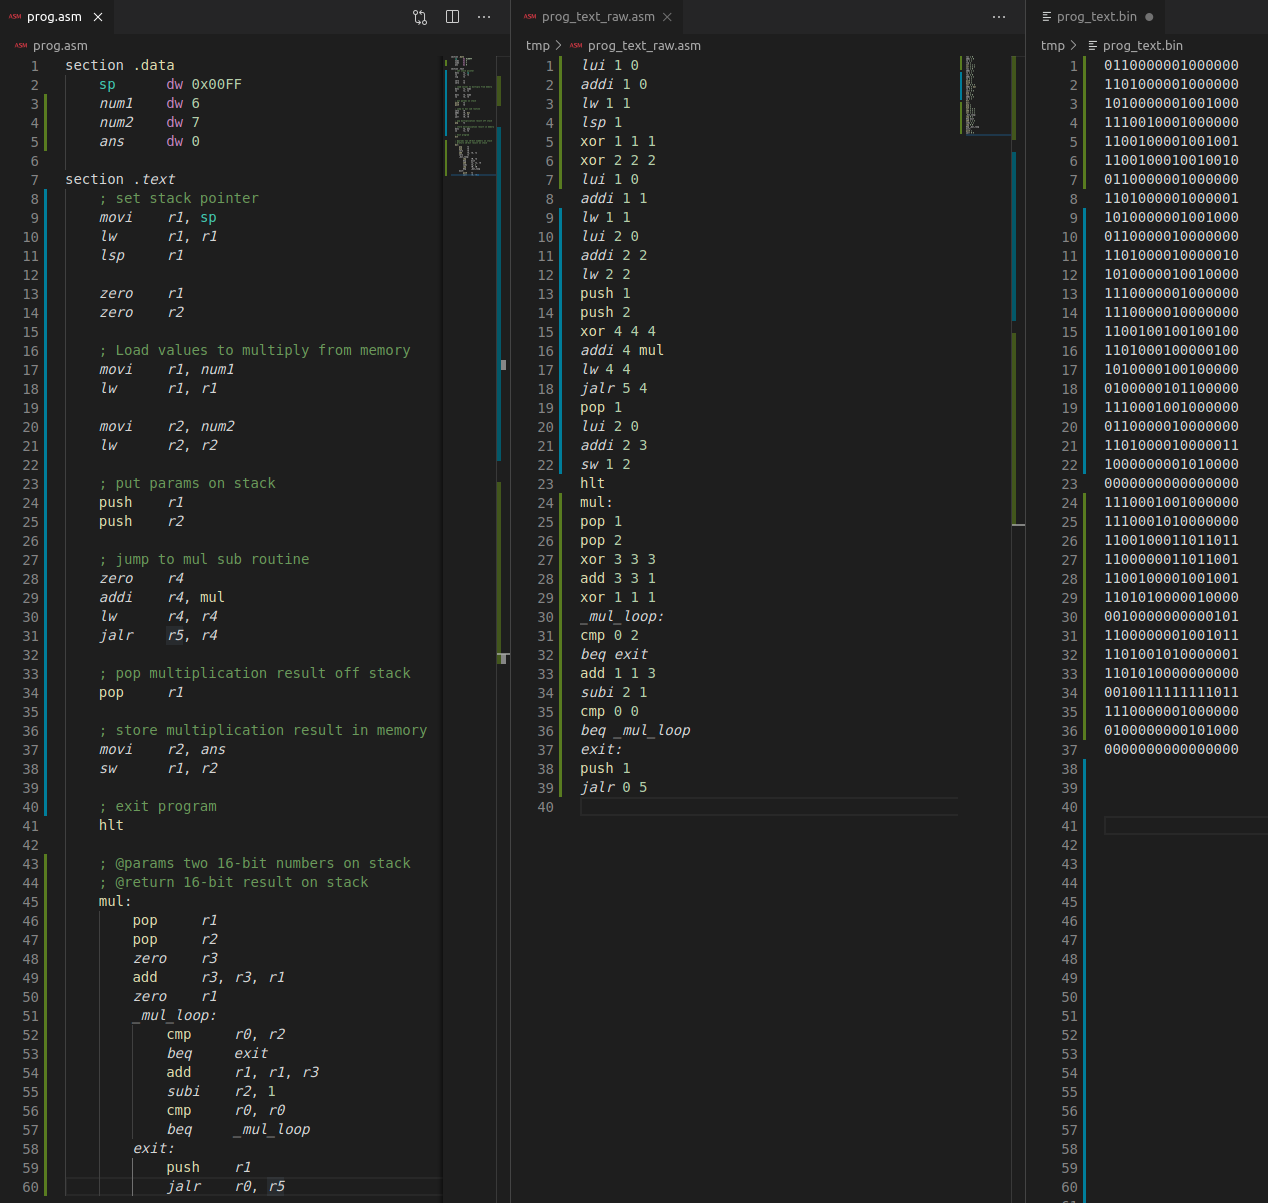
\includegraphics[width=5in]{img/test_prog.png}
		\caption{ Test Program }
		\label{fig:test_prog}
	\end{figure}

	A test program is written to demonstrate the functionality of system memory (Figure \ref{fig:test_prog}). The test program computes seven times six. The values of seven and six are loaded from memory multiplied and the result is written back to memory. The stack is used to pass data to and from the multiplication subroutine. The stack pointer is set to 255 at the beginning of the program. This test program adequately test all CPU memory functionality. 
	
	
	\begin{figure}[H]
		\centering
		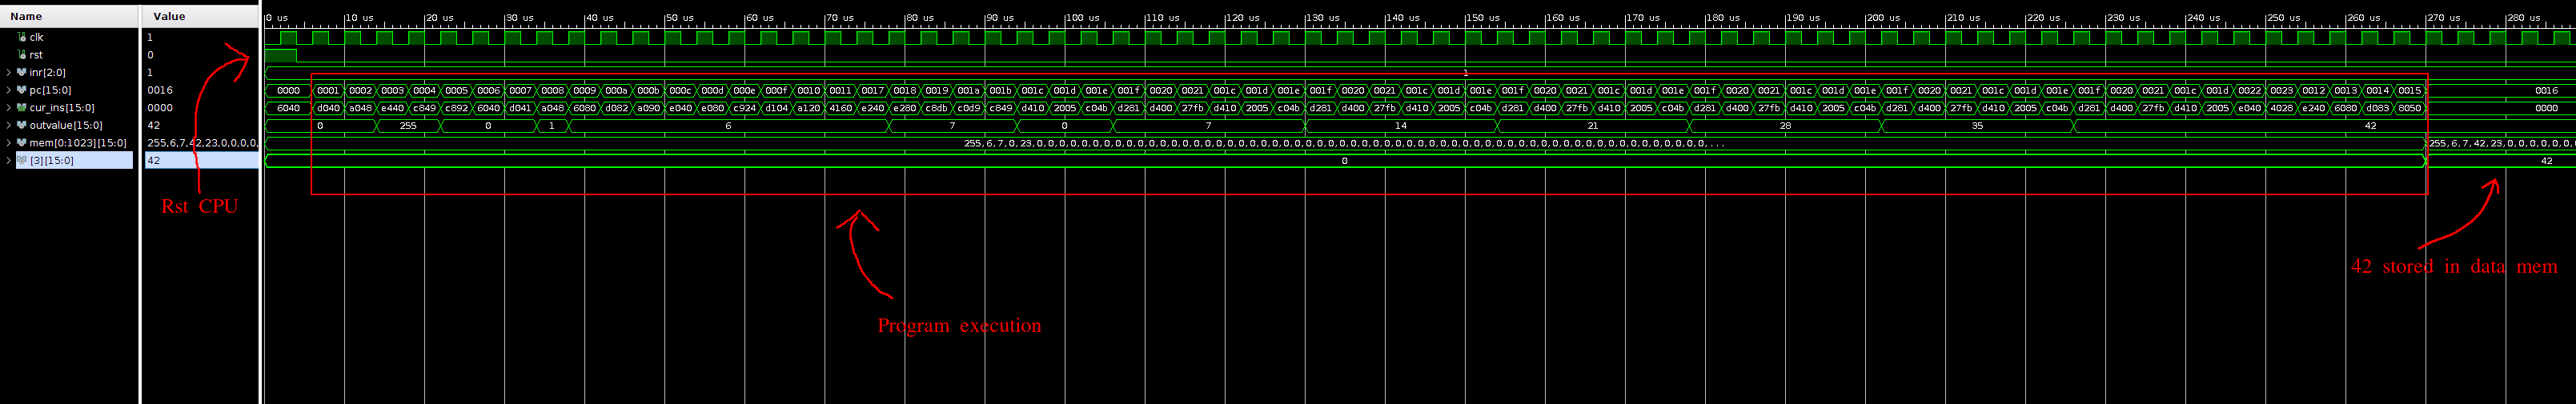
\includegraphics[width=7in]{img/prog_sim.png}
		\caption{ Test Program Simulation }
		\label{fig:test_prog_sim}
	\end{figure}

	\newpage

	The test program shown in Figure \ref{fig:test_prog} is simulated in Figure \ref{fig:test_prog_sim}. As shown by the Figure \ref{fig:test_prog_sim} annotations the ultimate answer 42 is computed and stored in memory at the end of the program. This final result 42 verifys that all the stack operations, loads, stores, and conditional / non-conditional jumps worked as intended. Figure \ref{fig:test_prog_sim2} shows the same content as Figure \ref{fig:test_prog_sim} but also displays all CPU control signals. 
	
	\begin{figure}[H]
		\centering
		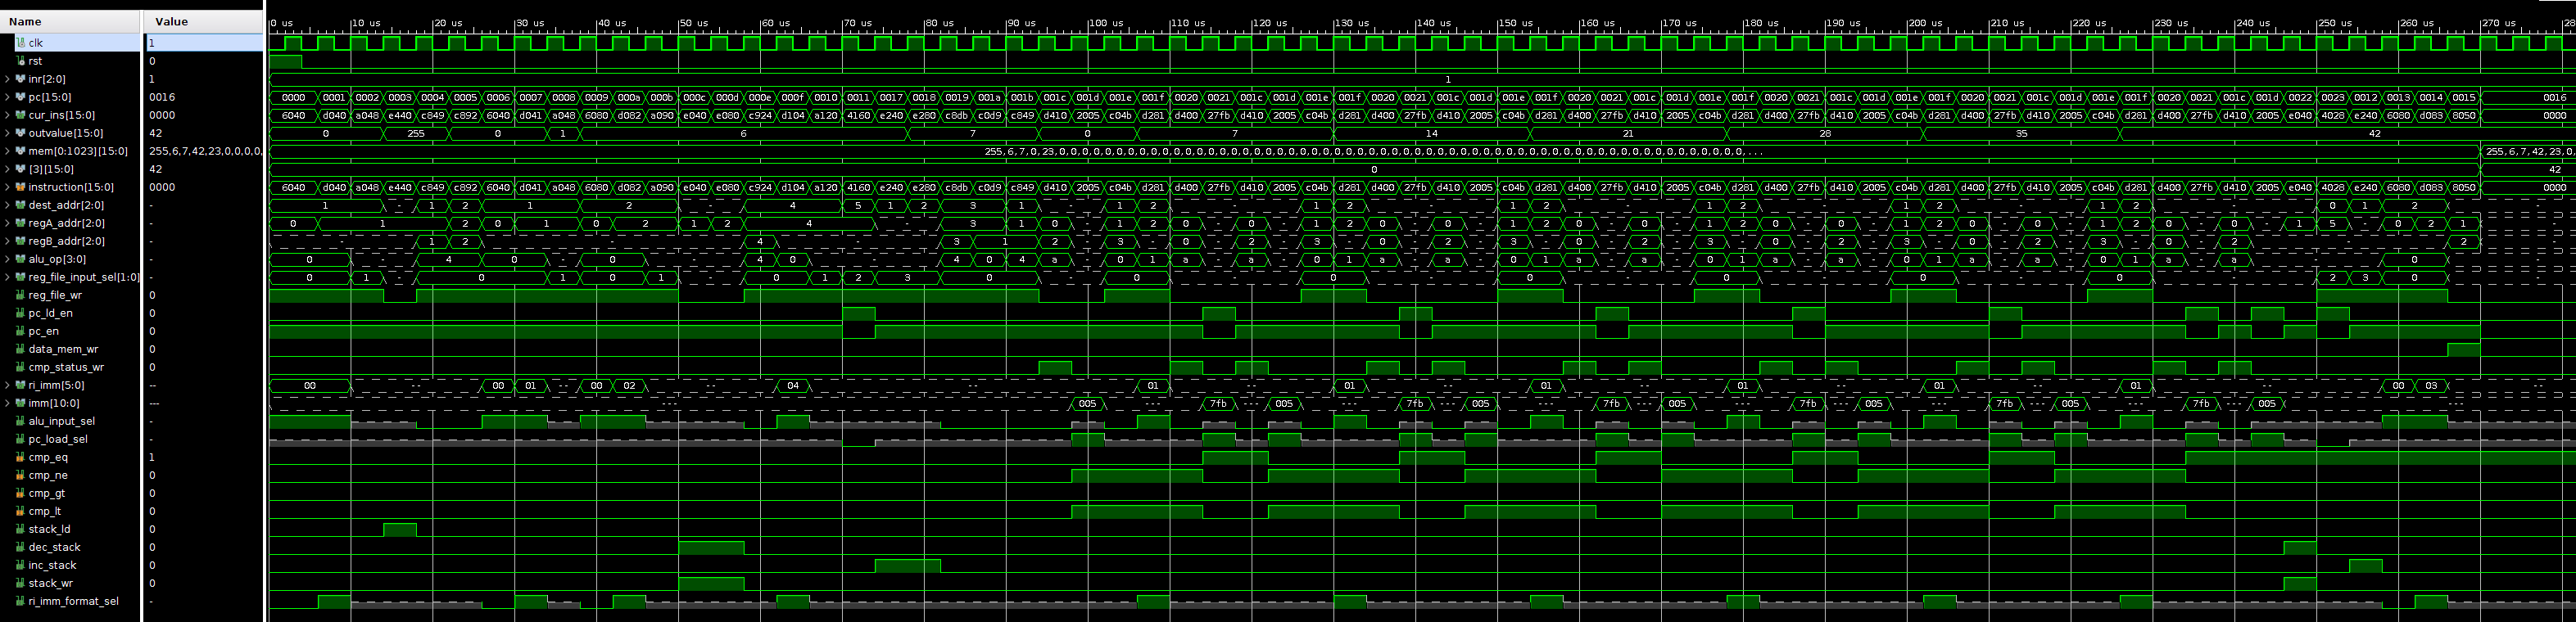
\includegraphics[width=7in]{img/test_prog2.png}
		\caption{ Test Program Simulation With Control Signals }
		\label{fig:test_prog_sim2}
	\end{figure}

\end{par}


\end{document}